\chapter{Data Management \& Data Access}

\section{HDFS}

The Hadoop Distributed File System, or HDFS for short, is a distributed File System engineered to run on any kind of hardware and to be easily scalable into huge clusters. Originally developed for Apache Nutch is now part of the Hadoop project, providing high fault-tolerance thanks to data replication and high throughput access to application data, making it suitable for Big Data applications.

\subsection{Architecture} 

HDFS has a master-slave architecture, comprised of two main components: a single \textbf{NameNode} which functions as a master and is in charge of the File System namespace management and the access control on its data by the clients and a list of \textbf{DataNodes} spread among the cluster's machines which handle the storage on the node they run on.\newline
HDFS interface, managed by the \textbf{NameNode} exposes a File System namespace and allows users to store data in files within a directory-based hierarchy, much like the regular File Systems used in general purpose machines; under the surface the file is split in one or more blocks which are then stored on a subset of \textbf{DataNodes} called rack.\newline The \textbf{NameNode} stores the metadata of the content of the whole File System and is responsible for the File System namespace operations over the files and directories and determines how blocks are mapped to the \textbf{DataNodes}.
The \textbf{DataNodes} serve the read and write requests sent by the File System's clients and can perform basic operations on the block (creation, deletion, copy) when so instructed by the \textbf{NameNode}.

\subsection{Replication} 

Exposing a File System built upon a cluster of many machines requires the technology to be reliable in case of a malfunction, since the chance of failure of the whole system is inherently greater if its functions depend on any of the single machines that comprise it. \newline Therefore to make sure that data is always available to clients, whenever a file is stored on the File System namespace and the \textbf{NameNode} chooses where to store the single blocks, it actually store the same block on more than one \textbf{DataNode} (the number depends on a configuration aptly named Replication Factor), in such a way that if any of those nodes become inaccessible for any reason, among all the others will always be a reachable copy of each block stored on it.\newline Secondly, the \textbf{NameNode} must always be available, therefore the HDFS provides a \textbf{Secondary NameNode}.

\subsection{Persistence}

The File System metadata, as previously stated, is managed by the \textbf{NameNode}. The \textbf{NameNode} uses a log to store persistently all the changes to these metadata, such as changing the replication factor, creating a new file, renaming an old one; the log, called EditLog, is stored in the host machine's File System. Similarly the state of the File System is stored on the machine's File System in a file called FsImage.\newline
In case of HDFS failure, on restart the \textbf{NameNode} will load in memory the FsImage and then apply all the transactions stored on EditLog, to return to the last safe state it was before failure.
\newline
If no failures occur and the \textbf{NameNode} is not restarted, FsImage will become stale while EditLog's size will continue to increase to unmanageable size, to cope with this problem, HDFS uses a \textbf{Secondary NameNode} whose object is to query EditLogs to the \textbf{Primary NameNode} at regular intervals, to update its own copy of FsImage accordingly and to then send its copy to the \textbf{Primary NameNode}.

\subsection{Robustness}

HDFS is designed to be reliable in the event of the three most common failures: \textbf{NameNode} failures, \textbf{DataNode} failure and network failures.

Each \textbf{DataNode} sends a heartbeat regularly to the \textbf{NameNode} to prove its liveness, the latter considers the formers without recent heartbeats dead and stop sending read and write requests to them until a new heartbeat arrives.\newline
While \textbf{DataNodes} failures may cause them to be dead, Network failures can cause alive \textbf{DataNodes} to lose their heartbeats and be considered dead.\newline
Whatever the root of the problem, the \textbf{NameNode} tracks the blocks that are now under replicated and marks them to be replicated as soon as it has available space on a machine that doesn't already have a copy of them.\newline
Checksums for each block of stored files make sure that corruption caused by faults in Nodes are spotted and their corrupted blocks rejected.\newline
As for \textbf{NameNode} problems, the secondary \textbf{Secondary NameNode} manages a consistent copy of FsImage and EditLog that functions as a backup in case of the corruption of the original ones. Nevertheless the \textbf{NameNode} is a single point of failure in the whole system; this is solved through High Availability, by providing a perfect another \textbf{NameNode}, which serves as a \textbf{Secondary NameNode} during downtime and as a \textbf{Primary NameNode} if the main one is not available.

\pagebreak
\section{YARN} \label{YARN}

\textbf{YARN (Yet Another Resource Negotiator)} is Hadoop's cluster and resource manager, whose fundamental idea is to split up the functionalities of resource management and job scheduling and monitoring into separate daemons: a global \textbf{Resource Manager (RM)} and per-application, either a single job or a DAG of jobs, \textbf{Application Master (AM)}.
\newline\newline
The \textbf{Resource Manager}, together with the \textbf{Node Manager (NM)}, forms the data computation framework: the first one is the ultimate authority that arbitrates resources among all the applications in the system, while the other is the per-machine framework agent who is responsible for containers, monitoring their resource usage and reporting it to the Resource Manager.
\newline\newline
The per-application Application Master is, in effect, a framework specific library and is tasked with negotiating resources from the Resource Manager and working with the Node Manager(s) to execute and monitor the tasks.

\subsection{Resource Manager}

The \textbf{Resource Manager}, the master component in YARN architecture, has two main components: the Scheduler and the Applications Manager.

The \textbf{Scheduler} is responsible for allocating resources to the various running applications subject to familiar constraints of capacities, queues etc. It performs no monitoring or tracking of status for the application and offers no guarantees about restarting failed tasks either due to application failure or hardware failures. 

Scheduling is performed based on the abstract notion of a Container incorporating elements such as memory, CPU, disk, network etc. which represent the resource requirements of the applications. It has a pluggable policy which is responsible for partitioning the cluster resources among the various queues, applications etc. The current schedulers such as the \textit{Capacity Scheduler} and the \textit{Fair Scheduler} would be some examples of plug-ins.

The \textbf{Applications Manager} is responsible for accepting job-submissions, negotiating the first container for executing the application specific Application Master and provides the service for restarting the Application Master container on failure. The per-application Application Master has the responsibility of negotiating appropriate resource containers from the Scheduler, tracking their status and monitoring for progress.

YARN supports the notion of resource reservation via a \textbf{Reservation System}, that allows users to specify a profile of resources over-time and temporal constraints (e.g., deadlines), and reserve resources to ensure the predictable execution of important jobs. The Reservation System tracks resources over-time, performs admission control for reservations, and dynamically instruct the underlying scheduler to ensure that the reservation is fulfilled.

\subsubsection{Schedulers}

There are two possible schedulers that can be used in a YARN cluster: \textbf{Capacity Scheduler} and \textbf{Fair Scheduler}. While the first one allows for multiple-tenants to securely share a large cluster by allocating resources in a timely manner under capacity constraints, the other allows for YARN applications to share cluster resources fairly.

\paragraph{Capacity Scheduler}

The Capacity Scheduler is designed to run Hadoop applications as a shared, multi-tenant cluster in an operator-friendly manner while maximizing the throughput and the utilization of the cluster.

Traditionally each organization has its own private set of computing resources that have sufficient capacity to meet the organization’s Service Level Agreement under peak or near-peak conditions. This generally leads to poor average utilization and overhead of managing multiple independent clusters, one per each organization. Sharing clusters between organizations is a cost-effective manner of running large Hadoop installations since this allows them to reap benefits of economies of scale without creating private clusters. However, organizations may be concerned about sharing a cluster because they are worried about others using the resources that are critical for their applications needs.

The Capacity Scheduler is designed to allow sharing a large cluster while giving each organization capacity guarantees. The central idea is that the available resources in the Hadoop cluster are shared among multiple organizations who collectively fund the cluster based on their computing needs. There is an added benefit that an organization can access any excess capacity not being used by others. This provides elasticity for the organizations in a cost-effective manner.

Sharing clusters across organizations necessitates strong support for multi-tenancy since each organization must be guaranteed capacity and safe-guards to ensure the shared cluster is impervious to a single rogue application or user, or sets thereof. The Capacity Scheduler provides a stringent set of limits to ensure that a single application or user or queue cannot consume disproportionate amount of resources in the cluster. Also, the Capacity Scheduler provides limits on initialized and pending applications from a single user and queue to ensure fairness and stability of the cluster.

The primary abstraction provided by the Capacity Scheduler is the concept of queues. These queues are typically set up by administrators to reflect the economics of the shared cluster.

The Capacity Scheduler supports the following features:

\begin{itemize}

\item \textbf{Hierarchical Queues} - Hierarchy of queues is supported to ensure resources are shared among the sub-queues of an organization before other queues are allowed to use free resources, thereby providing more control and predictability.

\item \textbf{Capacity Guarantees} - Queues are allocated a fraction of the capacity of the grid in the sense that a certain capacity of resources will be at their disposal. All applications submitted to a queue will have access to the capacity allocated to the queue. Administrators can configure soft limits and optional hard limits on the capacity allocated to each queue.

\item \textbf{Security} - Each queue has strict ACLs\footnote{ACL: Access Control List, a data structure holding the permissions on an object for each user.} which controls which users can submit applications to individual queues. Also, there are safe-guards to ensure that users cannot view and/or modify applications from other users. Also, per-queue and system administrator roles are supported.

\item \textbf{Elasticity} - Free resources can be allocated to any queue beyond its capacity. When there is demand for these resources from queues running below capacity at a future point in time, as tasks scheduled on these resources complete, they will be assigned to applications on queues running below the capacity (pre-emption is also supported). This ensures that resources are available in a predictable and elastic manner to queues, thus preventing artificial silos of resources in the cluster which helps utilization.

\item \textbf{Multi-tenancy} - Comprehensive set of limits are provided to prevent a single application, user and queue from monopolizing resources of the queue or the cluster as a whole to ensure that the cluster isn't overwhelmed.

\item \textbf{Operability}
    \begin{itemize}
    \item \textbf{Runtime Configuration} - The queue definitions and properties such as capacity and ACLs can be changed, at runtime, by administrators in a secure manner to minimize disruption to users. Also, a console is provided for users and administrators to view current allocation of resources to various queues in the system. Administrators can add additional queues at runtime, but queues cannot be deleted at runtime.
    
    \item \textbf{Drain applications} - Administrators can stop queues at runtime to ensure that while existing applications run to completion, no new applications can be submitted. If a queue is in STOPPED state, new applications cannot be submitted to itself or any of its child queues. Existing applications continue to completion, thus the queue can be drained gracefully. Administrators can also start the stopped queues.
    \end{itemize}

\item \textbf{Queue Mapping based on User or Group} - This feature allows users to map a job to a specific queue based on the user or group.

\item \textbf{Priority Scheduling} - This feature allows applications to be submitted and scheduled with different priorities. Higher integer value indicates higher priority for an application. Currently Application priority is supported only for FIFO\footnote{FIFO: First In First Out, a policy for the executions of jobs, the first job to come is the first to be served.} ordering policy.

\end{itemize}

\paragraph{Fair Scheduler}

Fair scheduling is a method of assigning resources to applications such that all of them get, on average, an equal share of resources over time. Hadoop is capable of scheduling multiple resource types:  the Fair Scheduler bases, by default, scheduling fairness decisions only on memory, but it can be configured to schedule with both memory and CPU. When there is a single application running, it uses the entire cluster, and when other applications are submitted, resources that free up are assigned to them, so that each one eventually gets roughly the same amount of resources. Unlike the default Hadoop scheduler, which forms a queue of applications, this lets short apps finish in reasonable time while not starving long-lived apps. It is also a reasonable way to share a cluster between a number of users. Finally, fair sharing can also work with priorities, which are used as weights to determine the fraction of total resources that each application should get.

The scheduler organizes apps further into "queues", and shares resources fairly between these queues. By default, all users share a single queue, named “default”. If an app specifically lists a queue in a container resource request, the request is submitted to that queue. It is also possible to assign queues based on the user name included with the request through configuration. Within each queue, a scheduling policy is used to share resources between the running apps. The default is memory-based fair sharing, but FIFO and multi-resource with Dominant Resource Fairness can also be configured. Queues can be arranged in a hierarchy to divide resources and configured with weights to share the cluster in specific proportions.

In addition to providing fair sharing, the Fair Scheduler allows assigning guaranteed minimum shares to queues, useful for ensuring that certain users, groups or production applications always get sufficient resources. When a queue contains apps, it gets at least its minimum share, but when the queue does not need its full guaranteed share, the excess is split between other running apps. This lets the scheduler guarantee capacity for queues while utilizing resources efficiently when these queues don’t contain applications.

The Fair Scheduler lets all apps run by default, but it is also possible to limit the number of running apps per user and per queue, useful when a user must submit hundreds of apps at once, or in general to improve performance if running too many apps at once would cause too much intermediate data to be created or too much context-switching. Limiting the apps does not cause any subsequently submitted apps to fail, only to wait in the scheduler’s queue until some of the user’s earlier apps finish.

The Fair Scheduler, just like the Capacity Scheduler, supports hierarchical queues. All queues descend from a queue named “root”. Available resources are distributed among the children of the root queue in the typical fair scheduling fashion. Then, the children distribute the resources assigned to them to their children in the same fashion. Applications may only be scheduled on leaf queues. Queues can be specified as children of other queues by placing them as sub-elements of their parents in the fair scheduler allocation file.

Additionally, the fair scheduler allows setting a different custom policy for each queue to allow sharing the queue’s resources in any which way the user wants: FifoPolicy, FairSharePolicy (default), and DominantResourceFairnessPolicy are built-in and can be readily used, but a custom policy can be specified by extending \texttt{\justify{SchedulingPolicy}} class. 

\subsubsection{Fault tolerance \& High Availability}

The Resource Manager is the central authority that manages resources and schedules applications running on YARN. Hence, it is potentially a single point of failure in a YARN cluster. 

They are thus needed functionalities that provide for down-time invisibility to end-users, keeping the RM functioning across restarts and remedying in case of node failures.

\paragraph{Non-work-preserving RM restart} RM will save the application metadata, together with credentials like security keys and tokens, when clients submit an application in a pluggable state-store, storing its status and diagnostics at completion. In case of RM outage, as long as the required information is available in the state-store, at restart, the RM can pick up the application metadata and re-submit the applications if they weren't already completed (failed, killed, or finished) before RM went down.

During the down-time of RM, Node Managers and clients will keep polling RM until it comes up. Once it does, a re-sync command is sent by the RM, killing all NM's managed containers, re-registering with RM, shutting down this way all the Application Masters. After RM restarts and loads all the application metadata, it will create a new attempt (i.e. Application Master) for each application not yet completed, re-kicking that application as usual.

\paragraph{Work-preserving RM restart} This type of restart focuses on re-constructing the running state of RM by combining the container status from Node Managers and container requests from Application Masters on restart: running applications won't be killed after RM restarts, and so applications will not lose their work because of RM outage. 

RM ensures the persistence of application state, reloading it on recovery and re-constructing the entire running state of the YARN cluster, whose major information comes from the RM scheduler which keeps track of all containers' life-cycle, applications' headroom and resource requests and queues' resource usage. 
Applications can simply re-sync back with RM and resume from where they were left off: RM recovers its own running state by taking advantage of the containers statuses sent from all NMs on re-registration, reconstructing the container instances and the associated applications' scheduling status by absorbing this information. 

In the meantime, AM needs to re-send the resource requests to RM because RM may lose the unfulfilled requests when it shuts down.

\paragraph{High Availability} Resource Manager HA is realized through an Active/Standby architecture: at any point of time, one of the RMs is Active, and one or more RMs are in Standby mode waiting to take over should anything happen to the Active. The trigger to transition-to-active comes from either the admin (through CLI) or through the integrated failover-controller when automatic-failover is enabled. When automatic fail-over is not enabled, admins have to manually transition one of the RMs to Active, using the \verb|yarn rmadmin| CLI, first transitioning the Active-RM to Standby and then the Standby-RM to Active.

In order to guarantee automatic fail-over, it's possible to use both an existing \textbf{Zoo\-keeper} cluster or the embedded \verb|ActiveStandbyElector|, acting as a failure detector and leader elector instead of a separate Zookeeper FailoverController daemon, to decide which RM should be the Active: when the Active goes down or becomes unresponsive, another RM is automatically elected to be the Active, taking then over.

When there are multiple RMs, the configuration (\verb|yarn-site.xml|) used by clients and nodes is expected to list all the RMs. Clients, Application Masters and Node Managers try connecting to the RMs in a round-robin fashion until they hit the Active RM. If the Active goes down, they resume the round-robin polling until they hit the “new” Active. This retry logic can be overridden by a user-specified fail-over provider.

\subsection{Node Manager}

The \textbf{Node Manager} is the slave component in YARN architecture and is responsible for launching and managing containers on a node. The Node Manager runs services to determine the health of the node it is executing on. The services perform checks on the disk as well as any user specified tests. If any health check fails, the Node Manager marks the node as unhealthy and communicates this to the Resource Manager, as part of the heartbeat between the NM and the RM, which then stops assigning containers to the node.

Just like the Resource Manager, the Node Manager has a \textbf{work-preserving restart} feature, that enables the Node Manager to be restarted without losing the active containers running on the node. At a high level, the NM stores any necessary state to a local state-store as it processes container-management requests. When the NM restarts, it recovers by first loading state for various subsystems and then letting those subsystems perform recovery using the loaded state. 

\pagebreak
\section{SQL: Hive}

Apache Hive is a relational database for Big Data, developed as a part of the Hadoop environment to provide fast access to huge data sets through its own query language, \textbf{HiveQL}, and through several possible execution engines such as Apache Tez, MapReduce and Apache Spark. Hive, as of recently, added  support for ACID transactions, making it viable as a data storage for more complex endeavours, including streaming applications.

\subsection{Components}

Hive architecture can be divided in five main components:

\begin{itemize}
    \item \textbf{Shell/UI}: Beeline is the frontend tool for interactive querying on the database. Hive supports connections via its own JDBC driver, allowing easy integration with clients and user applications.
    \item \textbf{Driver}: The component which receives the queries. This component implements the notion of session handles and provides execute and fetch APIs\footnote{API: Application Programming Interface, a set of functions and protocols provided to developers.} modeled on JDBC/ODBC interfaces.
    \item \textbf{Metastore}: It stores metadata about HDFS file locations and the table schemas, but also column and column type information and the serializers and deserializers necessary to read and write data.
    \item \textbf{Compiler}: It manages query parsing, planning and optimization, does semantic analysis on the different query blocks and query expressions generating, eventually, an execution plan with the help of the table and partition metadata looked up from the metastore. For what concerns the parsing, HiveQL is a SQL extension, compliant with the SQL:2011 standard.
    \item \textbf{Execution Engine}: Hive uses Apache Tez as a default execution engine  which allows low latency querying through its LLAP (Low Latency Analytical Processing) daemons: persistent processes running on YARN enabling the system to avoid the overhead caused by the container deployment for query executions. Other execution engines usable by Hive are, as already mentioned, MapReduce and Spark. The first one is needed, as of Hive 2.1, in order to use Hive Streaming API, while the other uses its own LLAP daemons, similarly to Tez, and still lags behind, performance wise.
\end{itemize}

\subsection{Hive Low Latency Processing on Tez}

Starting from Hive2, OLAP, OnLine Analytical Processing support has been introduced as default mode for query execution on top of Apache Tez.\\  
This functionality has been implemented on top of YARN where, while deploying the endpoint for the clients queries (HiveServer2), two applications are deployed: 

\begin{itemize}
    \item a Tez query coordinator application, which deals with a single query execution planning, a series of Map and Reduce operations, but also the concurrency of many queries, if needed;
    \item a Slider \footnote{\href{https://slider.incubator.apache.org/}{Apache Slider} is an application which allows dynamic deployment and monitoring of YARN applications} application that, together with the persistent daemons containers, deals with the actual processing of the single operation that needs to be executed.
\end{itemize}

With respect to the usual query execution, this architecture allows:

\begin{itemize} 
	\item a critical decrease in the latency caused by the creation of the YARN containers needed for the query execution, which is usually the biggest time consuming task.
	\item parallel and concurrent query execution, shared between all the daemons instances, taking also advantage of the In-Memory Cache of the single daemon, especially useful if different queries need to access the same data.
\end{itemize}

The introduction of LLAP/OLAP daemons provided Hive2 with an average 2600\% performance gain when compared to Hive1 using Tez, on a dataset of 1 TB \cite{hive2_on_tez}.

\subsection{HiveQL}

HiveQL, which stands for Hive Query Language, is a SQL:2011 compliant language used for query expressions in Hive. Together with all the features coming from the SQL standard, it introduces concepts like external tables and table bucketing in its DDL\footnote{DDL: Data Definition Language, subset of a grammar which specifies the syntactic rules for the creation and alteration of objects such as databases, tables and indices.}, together with the possibility to use User Defined Functions for custom aggregations and operators.

\subsubsection{Data Definition Language}

HiveQL Data Definition Language allows creation and alteration of databases, tables and indices.\\When it comes to DBs, the classic statements \verb|CREATE|, \verb|ALTER| \& \verb|DROP| are available for creation, alteration and deletion of databases, together with the possibility to specify ownership, filesystem location and other custom properties.\\
Concerning tables, Hive DDL provides the ability to define external tables, located in the filesystem somewhere other than on the default warehouse, which can be read and queried like a normal table. In addition, it is possible to define constraints on column keys, such as foreign and primary keys, partitioning, bucketing, skewing and sorting for optimization purposes. It allows to define the kind of deserialization Hive needs to use in order to read the data stored, according to their file format with the \verb|ROW FORMAT| clause.

For example, the statement

\begin{minted}{SQL}
    CREATE TABLE IF NOT EXISTS 
    log_table(id string, count int, time timestamp)
    PARTITIONED BY (date string)
    CLUSTERED BY id SORTED BY (count DESC) INTO 10 BUCKETS
    SKEWED BY id ON 3, 4, 10
    STORED AS ORC;
\end{minted}

creates a table named "log\_table", using the default database, stored in ORC format partitioned according to a certain user-input string "date", in 10 ORC files sorted in descending order, where values are skewed on the id values 3, 4 and 10.

\subsubsection{Data Manipulation Language}

HiveQL Data Manipulation Language allows to modify data in Hive through multiple ways:

\begin{itemize}
    \item \verb|LOAD| allows file loading into Hive tables from HDFS or local filesystem.  
    \item \verb|INSERT| allows to insert query results into Hive tables or filesystem directories. In case it's needed, it is possible to overwrite or insert them into a dynamically created partition. 
    \item \verb|UPDATE| and \verb|DELETE| allow to update or delete values in tables supporting Hive Transactions.
    \item \verb|MERGE| allows to merge files belonging to the same table, if it supports Hive Transactions.
    \item \verb|IMPORT| and \verb|EXPORT| allow importing and exporting of both table values and metadata, to use them with other DBMS.
\end{itemize}

\subsection{Warehouse}
HDFS is the default physical storage of database and tables in Hive, but support for S3 and any other HDFS compatible filesystems is available. Since all of the files are stored on a distributed filesystem, redundancy and fault tolerance are granted when it comes to data integrity. Hive default storage format is ORC, a compressed format able to decrease file size up to 78\% with respect to normal Text Files \cite{orc_format}.\\
Hive has built-in direct serialization and deserialization of CSV, JSON, AVRO and Parquet files as row formats, and allows to easily add custom SerDe\footnote{SerDe: Serialization/Deserialization} components.

\subsubsection{Hive Data Model}

Data in Hive is organized into 3 main abstractions: Tables, Partitions and Buckets.

\paragraph{Tables} These are analogous to Tables in Relational Databases. Tables can be filtered, projected, joined and unioned. Additionally all the data of a table is stored in a directory in its default warehouse, usually HDFS. Hive also supports the notion of external tables wherein a table can be created on pre-existing files or directories in HDFS by providing the appropriate location to the table creation DDL. The rows in a table are organized into typed columns similar to Relational Databases.
\paragraph{Partitions} Each Table can have one or more partition keys which determine how the data is stored, for example a table \texttt{T} with a date partition column \texttt{ds} had files with data for a particular date stored in the \texttt{<table location>/ds=<date>} directory in HDFS. Partitions allow the system to prune data to be inspected based on query predicates, for example a query that is interested in rows from \texttt{T} that satisfy the predicate \texttt{\justify{T.ds='2008-09-01'}} would only have to look at files in \texttt{\justify{<table location>/ds=2008-09-01/}} directory in HDFS.
\paragraph{Buckets} Data in each partition may, in turn, be divided into Buckets based on the hash of a column in the table. Each bucket is stored as a file in the partition directory. Bucketing allows the system to efficiently evaluate queries that depend on a sample of data (these are queries that use the SAMPLE clause on the table).
\newline
\par
Apart from primitive column types (integers, floating point numbers, generic strings, dates and booleans), Hive also supports arrays and maps. Additionally, users can compose their own types programmatically from any of the primitives, collections or other user-defined types. The typing system is closely tied to the SerDe and object inspector interfaces. Users can create their own types by implementing their own object inspectors, and using these object inspectors they can create their own SerDes to serialize and deserialize their data into HDFS files).\\
These two interfaces provide the necessary hooks to extend the capabilities of Hive when it comes to understanding other data formats and richer types. Built-in object inspectors like \verb|ListObjectInspector|, \verb|StructObjectInspector| and \verb|MapObjectInspector| provide the necessary primitives to compose richer types in an extensible manner. For maps (associative arrays) and arrays useful built-in functions like size and index operators are provided. The dotted notation is used to navigate nested types.

\subsection{Hive \& SQL Server 2016}

When it comes to enterprise-level solutions, every data warehousing product needs to be compared with the de-facto standard of this sector. Considering a pure Windows environments, Microsoft's SQL Server is the most widely used RDBMS and data warehouse.\newline

\subsubsection{Comparison}

A comparison has been set up in order to compare the capabilities of Hive with respect to SQL Server, using Hortonworks' TPC-DS\footnote{TPC Benchmark DS is a decision support benchmark that models several generally applicable aspects of a decision support system, including queries and data maintenance. The benchmark provides a representative evaluation of performance as a general purpose decision support system. TPC-DS Version 2 enables emerging technologies, such as Big Data systems, to execute the benchmark. Benchmark implementation: \href{https://github.com/hortonworks/hive-testbench}{https://github.com/hortonworks/hive-testbench}} Testbench implementation with a dataset of 30 GB, results averaged on 5 executions with machines with the following specifications and the following optimizations:
\newline

\begin{table}[!htb]
    \caption{Machine Specifications and Optimizations}
\begin{center}
    \begin{tabular}{|l|p{6cm}|p{5cm}|}
        \hline
        & Hive & SQL Server \\ \hline
        Specifications & 4 LLAP executors (4GB and 2 vCPU each) & 4 cores\\
        & Tez (512MB, 1vCPU) & 16GB RAM\\
        & Slider (512MB, 1vCPU) & Windows Server 2012 R2 \\
        & Total: 17GB, 5 core (10 vCPU) & \\ \hline    
        Optimizations & ORC Format storage, Partitioned tables & Clustered, suggested and ad hoc indices\\ \hline      
    \end{tabular}
\end{center}
\end{table}


Note: Tez and Slider containers, as mentioned in the previous chapter don't actually process any data and are used only for query orchestration.

\subsubsection{Results}

For a total of 65 queries executed, Hive is faster (1.5 to 1200 times) for 38 of them, while SQL Server is better in 19 query executions (1.5 to 54 times), while the remaining 8 queries display similar performances, standing inside the neighbourhood of 1.5x ratio.

Looking at the best results for both sides, we can see that Hive performs better with queries with many WHERE clauses and nested queries, while SQL Server performs better with queries with many \texttt{GROUP BY}, \texttt{SORT BY} and \texttt{JOIN} clauses.

\begin{table}[!htb]
    \begin{center}
            \caption{Hive top 3 best results}
        \begin{tabular}{|l|c|c|c|} \hline
            & Hive & SQL Server & Speedup factor\\ \hline
            query60 & 945 ms & 1.127.549 ms & 1193 \\ \hline
            query7 & 814 ms & 243.714 ms & 299 \\ \hline
            query26 & 1.083 ms & 80.997 ms & 74 \\ \hline
        \end{tabular}
    \bigskip
    \caption{SQL Server top 3 best results}
        \begin{tabular}{|l|c|c|c|} \hline
        & Hive & SQL Server & Speedup factor\\ \hline
        query95 & 37.762 ms & 1.104 ms & 34 \\ \hline
        query22 & 83.305 ms & 7.007 ms & 12 \\ \hline
        query72 & 134.611 ms & 40.043 ms & 3,3 \\ \hline
    \end{tabular}
    \end{center}
\end{table}

\subsubsection{Conclusions}

We can conclude that, generally, Hive applies to different use cases with respect to SQL Server. Whereas, Hive is suitable in scenarios where data sets are very big, where a distributed architecture can be used to scale and speed up the processing of huge swaths of data, SQL Server handles itself progressively worse as data set size increase, becoming an unideal fit in this case. Still, if the data set is limited in size, a single machine architecture is certainly more cost-effective and gives out good performances, having a better and more mature and optimized ACID transactions handling if required.

\section{Cassandra}

More often than not, in a big data environment, the classic relational model is not sufficient to describe the data ingested and processed, since they can be in any non-structured format, from raw text to images or complex JSONs and thus need properly modelled data structures and an horizontally scalable architecture able to handle huge data with a finer control over availability.

Many NoSQL data stores compromise consistency (in the sense of the \textbf{CAP theorem} \cite{Gilbert:2002:BCF:564585.564601}) in favor of availability, partition tolerance, and speed, while offering a concept of "eventual consistency" in which database changes are propagated to all nodes \textit{eventually} (typically within milliseconds) so queries for data might not return updated data immediately or might result in reading data that is not accurate, a problem known as \textit{stale reads}.

One of the most widely used NoSQL DBMS in Hadoop environments is \textbf{Cassandra} , a wide column data store which favours Availability and Partition Tolerance, in spite of Tuneable Consistency, highly scalable and with \textit{no single point of failure} \cite{Lakshman:2010:CDS:1773912.1773922}. Other NoSQL solutions are \textbf{HBase} a wide column key-value data store distributed on HDFS, which favours strong consistency in spite of availability, and \textbf{MongoDB}, a distributed document store.

\subsection{Architecture}

\begin{figure}[h]
    \centering
    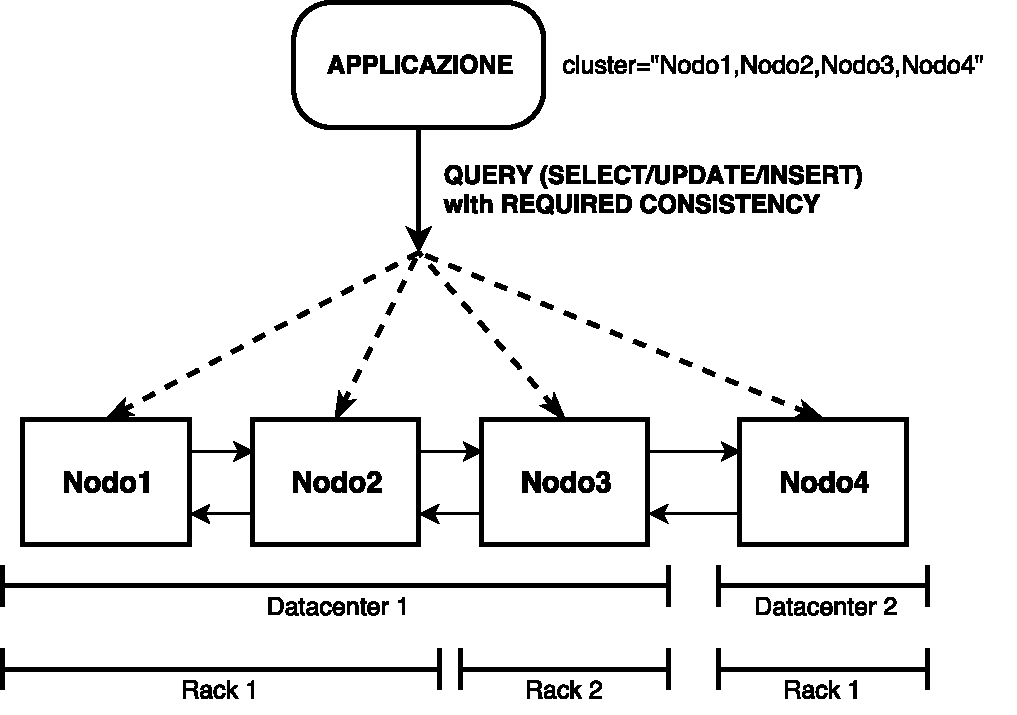
\includegraphics[width=0.7\linewidth]{Figures/cassandra_arch}
    \caption{An overview of Cassandra Architecture}
    \label{fig:cassandraarch}
\end{figure}


Cassandra's architecture revolves around all of the cluster nodes being equal, thus eliminating the need of a master-slave architecture which implicitly introduces a point of failure in the availability. Cassandra’s design was influenced by \textbf{Staged Event-Driven Architecture}, SEDA. \textbf{SEDA} is a general architecture for highly concurrent Internet services \cite{Welsh:2001:SAW:502059.502057} where a single operation may start with one thread, which then hands off the work to another thread, which may hand it off to other threads. Work is subdivided into what are called stages, basic units of work, and the thread pool associated with the stage determines execution. This design means that Cassandra is better able to manage its own resources internally because different operations might require disk I/O, or they might be CPU-bound, or they might be network operations, so the pools can manage their work according to the availability of these resources.

\paragraph{Data Center \& Racks} Cassandra is frequently used in systems spanning physically separate locations. Cassandra provides two levels of grouping that are used to describe the topology of a cluster: data center and rack. A rack is a logical set of nodes in close proximity to each other, on physical machines in a single rack of equipment. A data center is a logical set of racks, located in the same building and connected by reliable network. Out of the box, Cassandra leverages the information provided by the configuration of the cluster’s topology to determine where to store data, and how to route queries efficiently. Cassandra tries to store copies of data in multiple data centers to maximize availability and partition tolerance, while preferring to route queries to nodes in the local data center to maximize performance.

\paragraph{Partition Tolerance \& Node Communication} To support decentralization and partition tolerance, Cassandra uses a gossip protocol that allows each node to keep track of state information about the other nodes in the cluster. The gossiper runs every second on a timer. \textbf{Gossip protocols} (sometimes called “epidemic protocols”) generally assume a faulty network, are commonly employed in very large, decentralized network systems, and are often used as an automatic mechanism for replication in distributed databases.
When the gossiper determines that another endpoint is dead, it \textit{convicts} that endpoint by marking it as dead in its local list and logging that fact.
Failure detection is robustly supported through the \textbf{Phi Accrual Failure Detection algorithm} \cite{hayashibara2004spl}, which is based on the ideas that failure detection should be flexible, decoupling it from the monitored application, and that a traditional heartbeat approach is naive and should be improved via a \textit{suspicion level}, which is the confidence of an actual node failure.
An additional component in Cassandra architecture is the \textbf{Snitch}, which is used to determine relative host proximity in a cluster and gather information about network topology to efficiently route requests, both writes and reads, and in its dynamic implementation uses a modified version of the Phi failure detection mechanism used by gossip.

\paragraph{Consistency Levels} Cassandra's tuneable consistency make it so that database performances could span from a strong consistency, where each node need to acknowledge each write, to weak consistency, where a single node is sufficient to confirm a write. A consistency level is specified for each read or write query: the higher level of consistency the higher number of nodes or replicas must be acknowledged to the client. Levels go from \texttt{ANY}, \texttt{ONE}, \texttt{TWO} and \texttt{THREE}, considered weak consistency, to \texttt{QUORUM} and \texttt{ALL}, considered strong.

\paragraph{Caching and Tables} Cassandra stores data both in memory and on disk to provide both high performance and durability. When a write operation is performed, it’s immediately written to a \textbf{commit log}. The commit log is a crash-recovery mechanism that supports Cassandra’s durability goals. A write will not count as successful until it’s written to the commit log, to ensure that, if a write operation does not make it to the in-memory store, the \textbf{Memtables}, it will still be possible to recover the data. Each memtable contains data for a specific table and when the number of objects stored in the memtable reaches a threshold, the contents of the memtable are flushed to disk in a file called an \textbf{SSTable}, a compacted representation of the memtable, and a new memtable is then created.

Cassandra provides three forms of caching: the \textbf{key cache}, storing a map of partition keys to row index entries, facilitating faster read access into SSTables stored on disk; the \textbf{row cache}, caching entire rows, that can greatly speed up read access for frequently accessed rows, at the cost of more memory usage, and the \textbf{counter cache} used to improve counter performance by reducing lock contention for the most frequently accessed counters.

\paragraph{Storage} A \textbf{partitioner} determines how data is distributed across the nodes in the cluster. Each row has a partition key that is used to identify the partition. A partitioner, then, is a hash function for computing the token of a partition key. Each row of data is distributed within the ring according to the value of the partition key token. Furthermore, each node serves as a replica for different ranges of data: Cassandra replicates data across nodes in a manner transparent to the user, and the \textbf{replication factor} is the number of nodes in the cluster that will receive copies (replicas) of the same data.
The orchestration of Cassandra's storage management is done through internal control mechanisms such as the \textbf{Storage Engine}, which manages all aspects of table storage, including commit logs, memtables, SSTables, and indexes.

\subsection{Data Model \& CQL}

With respect to classic relational database design principles, which favours a normalized design of the database, in order to efficiently design a data model in Cassandra, it must be taken into account that \texttt{JOIN}s cannot be performed on Cassandra as much as that there's no concept of referential integrity. It's favourable to use denormalized tables, modelled with a \textit{Query-first design}, with storage and sorting being design decisions.\\
\\
The basic Cassandra data structures are \textbf{columns}, \textbf{rows}, \textbf{tables}, \textbf{keyspaces} and \textbf{clusters}. The \textbf{column} is the most basic unit of data structure in the Cassandra data model, containing a name and a value of a particular type specified when the column is defined. Each column value contains \textbf{timestamps}, generated each time a value is updated, used by Cassandra to keep data current. In addition, a \textbf{Time To Live} can be configured to guarantee data deletion after the specified amount of time. A \textbf{row} is a container for columns, referenced by a primary key, a uniquely identifying column value. A \textbf{table} is a container for an ordered collection of rows, each of which is itself an ordered collection of columns. The ordering is determined by the columns, which are identified as keys. A \textbf{keyspace} is the outermost container for data in Cassandra, corresponding closely to a relational database. In the same way that a database is a container for tables in the relational model, a keyspace is a container for tables in the Cassandra data model. Like a relational database, a keyspace has a name and a set of attributes that define keyspace-wide behavior, while a \textbf{cluster} is a container for keyspaces that spans one or more nodes.\\
\\
Cassandra offers a SQL-like expressive query language, which supports all of the typical operations that can be done on a relational database, from creating tables and keyspaces, through \texttt{CREATE} queries, to \texttt{INSERT}ions and \texttt{UPDATE}s. The creation of a table must specify a type for each column name: types range from numeric data types (\texttt{int, bigint, smallint, tinyint, varint, float, double decimal}) to text types (\texttt{\justify{text, varchar, ascii}}) and time and identity data types (\texttt{timestamp, date, time, uuid, timeuuid}), but include also simple data types such as \texttt{boolean}, \texttt{blob}, binary large objects, \texttt{inet}, \texttt{counter} and collections such as \texttt{set}, \texttt{list} and \texttt{map}.

Users can define inside each keyspace their own types, composing them with the aforementioned basic types, making sure that if a collection type is used in a User Defined Type, it should be marked as frozen, a forward compatibility flag introduced to make sure that individual attributes will be accessible with an \textit{unfreeze} mechanism, once Cassandra will support it.